\documentclass[12pt]{article}
\usepackage[utf8]{inputenc}
\usepackage{float}
\usepackage{amsmath}
\usepackage{graphicx}

\usepackage[hmargin=3cm,vmargin=6.0cm]{geometry}
%\topmargin=0cm
\topmargin=-2cm
\addtolength{\textheight}{6.5cm}
\addtolength{\textwidth}{2.0cm}
%\setlength{\leftmargin}{-5cm}
\setlength{\oddsidemargin}{0.0cm}
\setlength{\evensidemargin}{0.0cm}

%misc libraries goes here


\begin{document}

\section*{Student Information } 
%Write your full name and id number between the colon and newline
%Put one empty space character after colon and before newline
Full Name :  Murat TOPAK\\
Id Number :  2036218\\

% Write your answers below the section tags
\section*{Experiment 1,2}
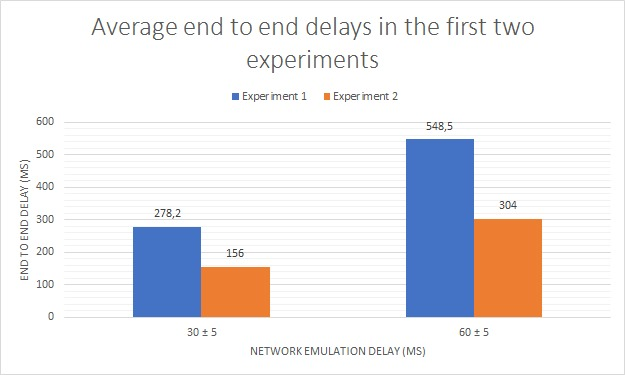
\includegraphics[scale=0.8]{graph.jpg}
\\


To begin with, the desired graph has two axes. The x-axis shows the network emulation delay with respect to the normal distribution in milliseconds while the y-axis reveals informatiıon about end to end delays, again in milliseconds. Two different bar colors distinguish between the first two experiments. Experiment 1 is the one with the path T1-G-T2-T3, and Experiment 2 has the path T1-G-U2-U3. These can be verified from the topology.
The end to end delay values above the bars represent the averages of samples. The sample size is 100 in these two experiments. 
\\

The 95\% confidence interval is computed from the formula on mathsisfun.com/data/confidence-interval.html. However, there are not any error bars in the graph to indicate the confidence intervals because such an introduction would seem so small compared to the rest of the figure. Therefore, the intervals are given as text below. 
\\

[278.2 $\pm$ 1.614452], [156 $\pm$ 1.97372], [548.5 $\pm$ 1.56996], [304 $\pm$ 2.09524]
\\\\

Now that the graph has been introduced, the findings can be explained.
As can be seen from the figure, there are two experiments conducted.
The shorter bars of course belong to the second experiment since its path involves UDP rather than TCP to some extent. At this point, let's apply our code's way of measurement and try to understand the average values with the emulation delays.
\\

The script residing on the client side(T1) sends a signal to the server(U3 or T3), and waits for a feedback. Therefore, all the measurement takes place when the packet travels back from server to the client. For example, the feedback path (U3-U2-G-T1) is followed in experiment 2.
\\

UDP is a very straightforward protocol compared to TCP; there is no handshake, no reliability. Thus getting a smaller value for the path involving UDP made sense, it was expected to be faster. Besides, from U3 to U2 and U2 to G are almost two emulation delays in total. On the other hand, the three way handshake of TCP requires almost three emulations delay for G-T1 communication, thus we have 5-emulation-delay end to end delay for experiment two.
\\

When the nodes implementing UDPs are turned into TCPs, as in experiment 1, there is an addition to the previously found 5-emulation-delay. In both TCP and UDP, the data is sent to the destination. However, TCP does a little more work than UDP. It establishes a connection before sending the packets so for each node turned into TCP, there is a 2-emulation-delay addition. Hence, 5 + 2*2 = 9-emulation-delay time passes in the experiment 1. When the average values of the emulation delays are substituted, we get very close to the real values. For example, 5x and 9x gives us 150 and 270 when x is 30. The experiments find these values as 156, and 278,2. Having used the normal distribution model, this deviation is expected, and tells us the approximation with only the means can only be a rough one.
\\

In summary, the experiments 1,2 showed us TCP adds a significant amount of delay compared to the UDP, especially when the delay at the sides of a link is in the order of tens of milliseconds.\\
\section*{Experiment 3,4}
To measure the packet losses in the last two experiments, the idea was to send 10,000 messages from client to server with unique IDs from 0 to 9999. Then the script running on each node would print the ID of each received message. The ones that don't get to print at this point are the losses. The experimental data collected with this method suggests this method responds to the changes in the packet loss percentage values correctly. Check out the figures below.
\\\\
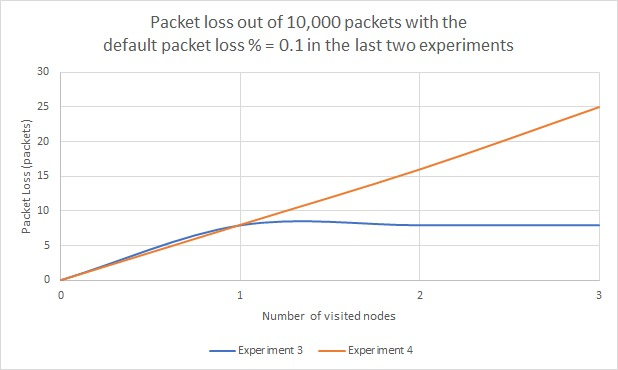
\includegraphics[scale=0.8]{graph2.jpg}
\\\\\\
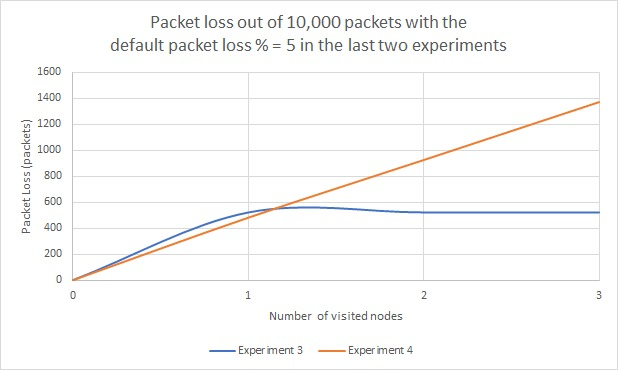
\includegraphics[scale=0.8]{graph3.jpg}

The graphs have two axes. The number of visited nodes lies on the x-axis. The y-axis shows the number of packets lost out of a sample of size 10,000. Experiment 3 starts with UDP, but turns into TCP after the first node. On the other hand, experiment 4 communicates with UDP all the time. These can be verified from the topology.
\\

The graphs reflect accurately the difference between two experiments. For instance, note the same packet loss experienced on the first node during both experiments. However, since experiment 3 makes use of TCP after the first node, it benefits from its reliability. Therefore, no more losses after the first step in experiment 3. This, however, is not the case for experiment 4. After the first node, it still communicates via UDP, so there are losses again and again in the following nodes. In terms of numbers, when the packet loss percentage was 0.1 and 5, experiment 3 only lost 8, and 521 packets respectively, out of 10,000 packets. On the other hand, experiment 4 had a linear fashion so the packet loss increased in each step. It was 8-16-25, and 483-928-1375, again respectively for the packet loss percentage values 0.1 and 5.
\\

For the sake of the experiments, there was a delay between requessts so that the drops related to buffer overflows did not misguide us. The conclusion here is that TCP tries its best to deliver a packet, while UDP drops packets without a care.


\section*{NTP}
While trying to calculate the end to end delay, we realized that the clocks should have been synchronized in order for the experiments to be accurate. Hence, NTP was installed and configured to achieve the 0ms/0ms clockdiff between the client and server.




\section*{Design}
Any other detail related to the structure and organization of the code can be found in the source codes as comments, or in the README file. This includes routing tables, threading, etc. Otherwise, this report would lose its high level of abstraction.





\end{document}

​
